% \section{Розвиток ресурсного центру УНГ на основі суперкомп'ютера СКІТ}

Важливим фактором розвитку і популяризації грід-технологій в Україні є наявність значних обчислювальних ресурсів у грід-інфраструктурі УНГ. Зокрема цього вимагає задача інтеграції України в європейський грід-простір~\cite{erevan-grid-2013}. На сьогоднішній день комплекс СКІТ надає в УНГ найбільший обсяг як обчислювальних ресурсів, так і ресурсів збереження. Проте розвиток технологій вимагає постійного оновлення як обладнання, так і системного та прикладного програмного забезпечення.


\section{Забезпечення надійності основних сервісів суперкомп'ютера}

В 2015 році EGI підвищило вимоги до надійності сервісів грід-сайтів. Тепер показник їх доступності (відношення часу, коли сервіси сайта проходять тести без помилок, до всього часу) має бути не меншим за 95\%. Тому постала задача підвищення надійності апаратної складової грід-сервісів, а також їх мобільності, тобто можливості швидкого перенесення всіх складових грід-сервісів кластера з несправного обладнання на справне.

Першим етапом цих робіт було перенесення всіх грід-серверів у віртуальні контейнери.  Було створено дослідний сервер-носій, на якому розміщувались всі віртуальні машини, необхідні для роботи ARC.

Дослідна експлуатація протягом 2014--2018 рр показала беззаперечні переваги такого рішення:

\begin{itemize}
\item можливість живої міграції, тобто перенесення віртуальної машини на резервний сервер-носій без перерви у наданні сервісів.
\item можливість "м'якого" оновлення проміжного ПЗ гріда. Оновлення відбувається не у робочій віртуальній машині, а у її копії. Коли оновлення готове, одна машина вимикається, а інша вмикається. А при появі якихось проблем з новим ПЗ, попередні версії сервісів відновлюються за декілька секунд.
\item відсутність жорсткої прив'язки до обладнання дозволила полегшити проведення планового та непланового технічного обслуговування серверів, і відповідно, підвищити надійність.                                                                                                                                                                              \end{itemize}

У 2016 році було проведено роботи з віртуалізації обчислювальних вузлів з черг моніторингу і діагностики.

Крім того, були оновлені ключові елементи інфраструктури -- кондиціонери та системи безперебійног живлення, що дозволить і надалі підтримувати високі стандарти надійності грід-сервісів.


\section{Віртуалізація вузлів діагностичного розділу грід-сайта}

До діагностичного розділу кластера грід-сайта входять вузли та черги, що виконують задачі систем моніторингу гріда. Ці задачі є придатними до віртуалізації, оскільки не потребують значних об'ємів пам'яті та процесорних ресурсів.  Це зумовлюють два фактори: 
\begin{enumerate}
\item підвищені вимоги до надійності цих вузлів, оскільки результати тестів на цих вузлах визначають оцінки кластера вцілому;
\item мінімальне обчислювальне навантаження при прохдженні теста.
\end{enumerate}

Було проведено аналіз технологій віртуалізації та виконано перенесення обчислювальних вузлів черги моніторингу у віртуальні контейнери. І таким чином зроблено внесок у вирішення задач підвищення енергоефективності обчислювального комплекса та підвищення його надійності.


\section{Інтеграція грід-сайта СКІТ до проекту ALICE}

Проект ALICE є одним з основних проектів Великого адронного коллайдера. Задачі обробки даних екперимента розподіляються по обчислювальним кластерам за допомогою грід-технологій та спеціалізованих віртуальних машин VOBOX. 

У роботі виконано роботи з узгодження системного ПЗ кластера СКІТ з потребами проекта ALICE, виконано встановлення та налагодження віртуального контейнера з сервісами VOBOX, отримання необхідних сертифікатів.

\begin{figure}
 \centering
 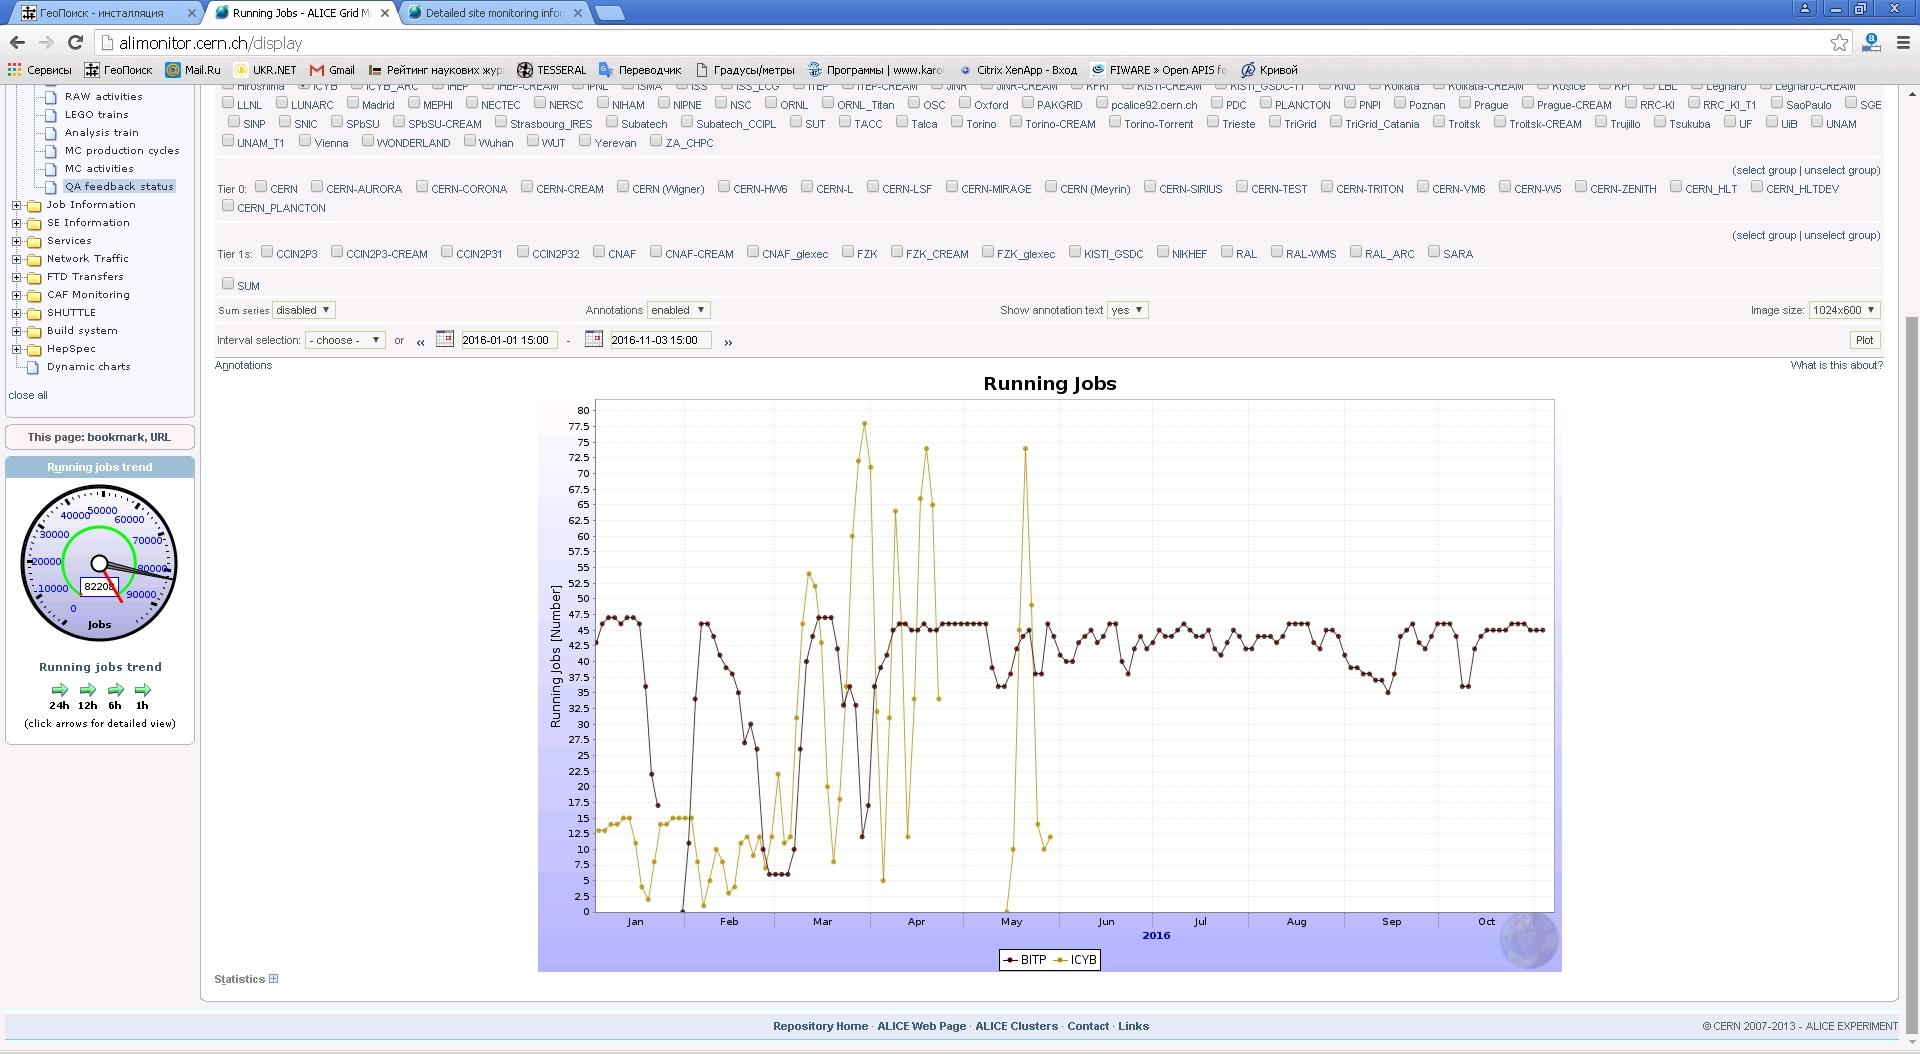
\includegraphics[width=14cm]{alice-stats.jpg} 
 \caption{Моніторинг проекта ALICE}
 \label{fig:alicemon}
\end{figure}

Крім того, проведено тестування роботи кластера з потоком реальних задач ALICE~\ref{fig:alicemon}.
